\documentclass[a4paper,11pt]{article}
\usepackage[polish]{babel}
\usepackage[OT4]{fontenc}
\usepackage[utf8]{inputenc}
\usepackage{graphicx}

\begin{document}

\title{Sprawozdanie ze sprawdzianu z PWI}
\author{Mikołaj Balwicki}
\date{\today}
\maketitle

\section{Zadanie 1}
Wygenerowałem klucze, wysłałem klucz publiczny na serwer i zalogowałem się z jego pomocą.\\
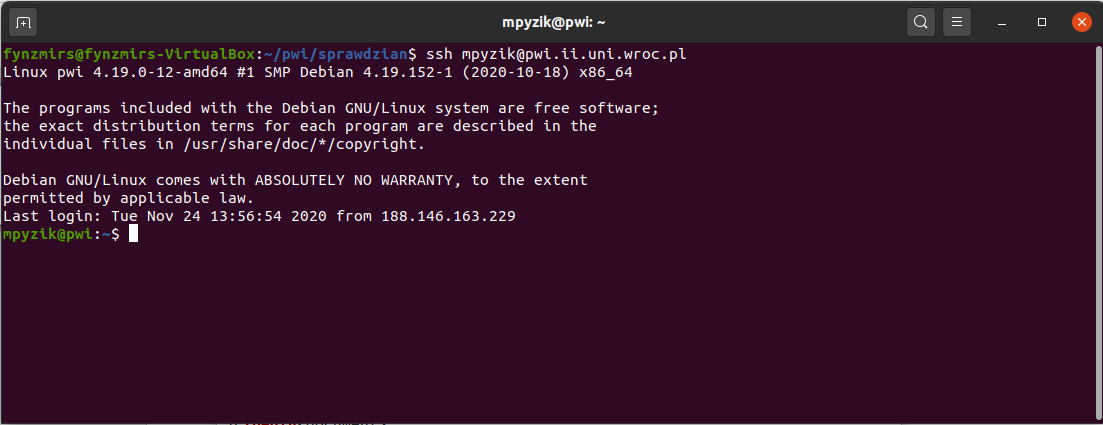
\includegraphics[width=\textwidth]{logowanie.png}

\section{Zadanie 2}
Ciąg liczb wygenerowałem komendą seq.\\
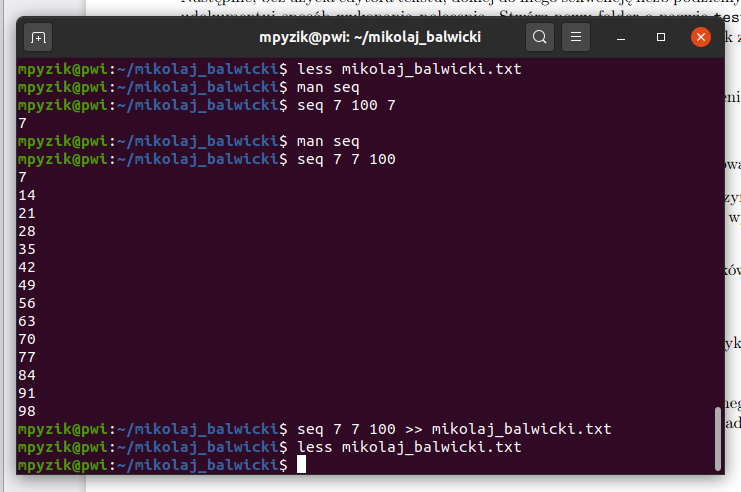
\includegraphics[width=\textwidth]{seq.png}\\
Na koniec pobrałem ten plik na swój komputer\\
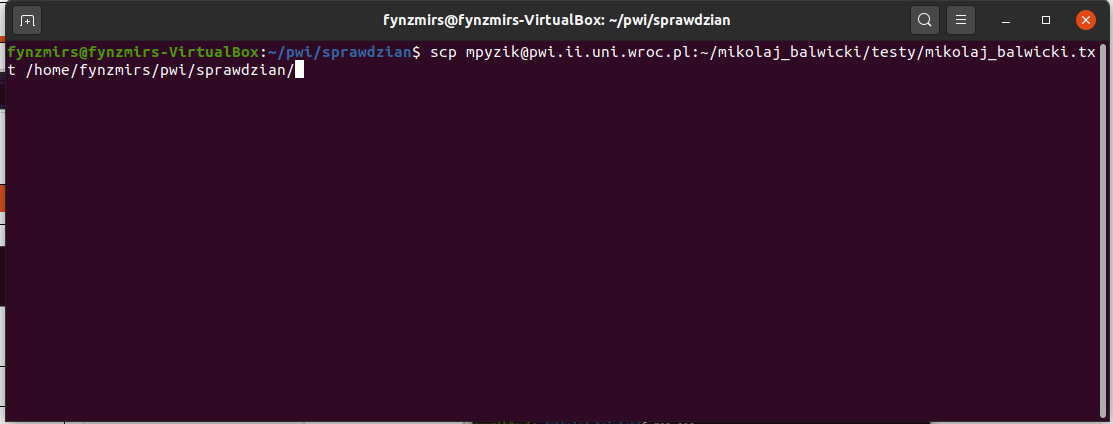
\includegraphics[width=\textwidth]{scp.png} 

\section{Zadanie 3}
\subsection{Tworzenie plików}
Pliki stworzyłem zgodnie ze sposobem podanym w treści zadania.\\
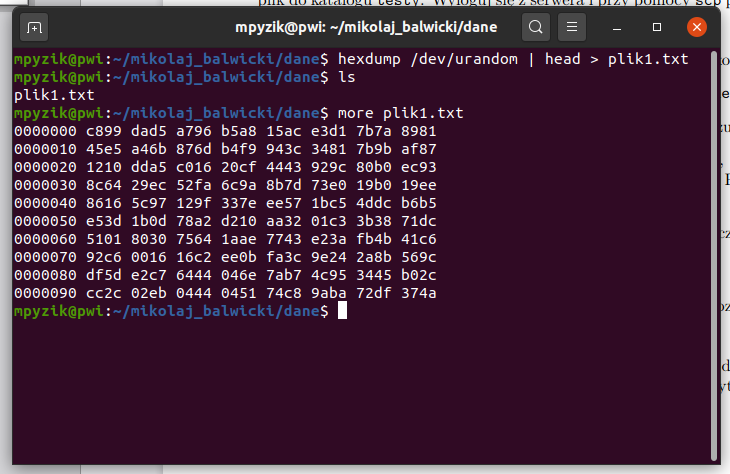
\includegraphics[width=\textwidth]{tworzenie_plikow.png}

\subsection{Sklejanie plików}
Pliki skleiłem z użyciem polecenia cat.\\
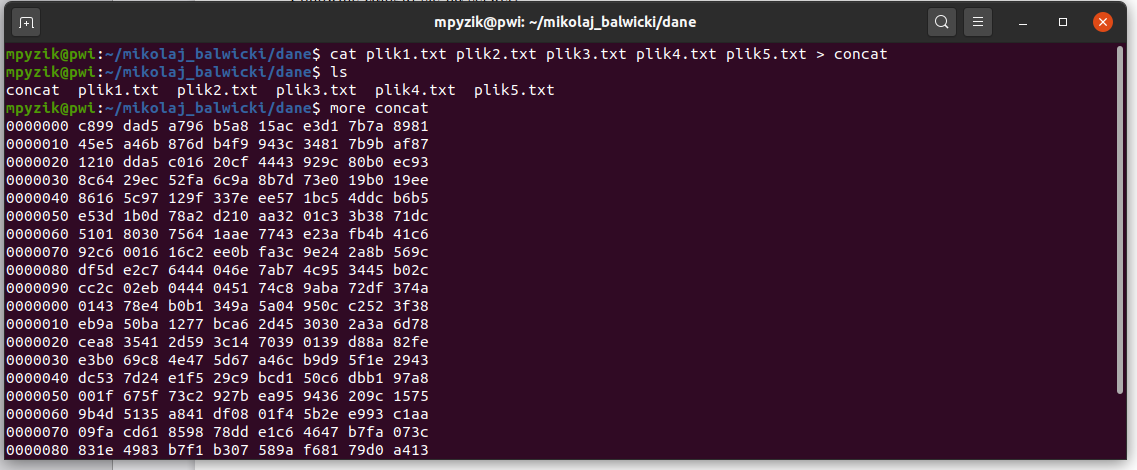
\includegraphics[width=\textwidth]{concat.png}

\subsection{Grep}
Próbowałem odnaleźć linie pasujące do wzoru, ale takich nie było.\\
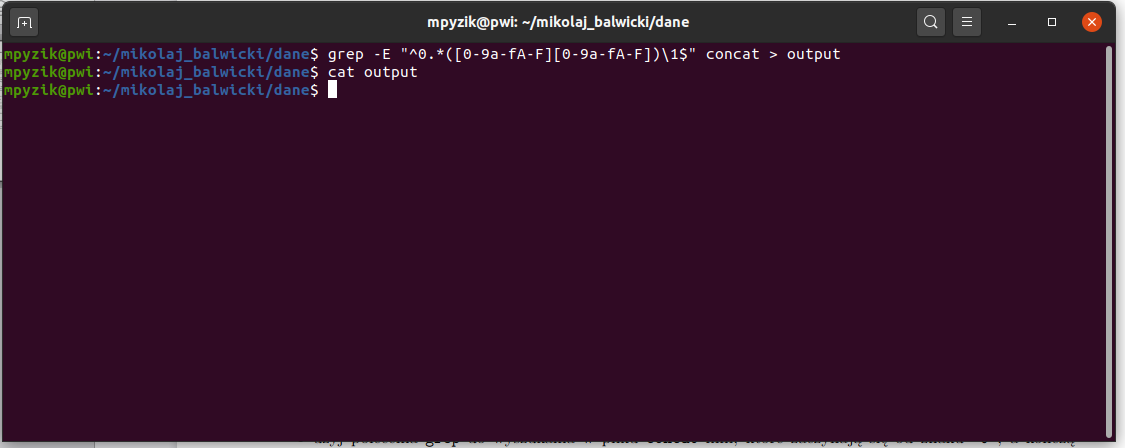
\includegraphics[width=\textwidth]{grep.png}

\subsection{Liczenie linii}
Skorzystałem z polecenia wc z odpowiednią flagą.\\
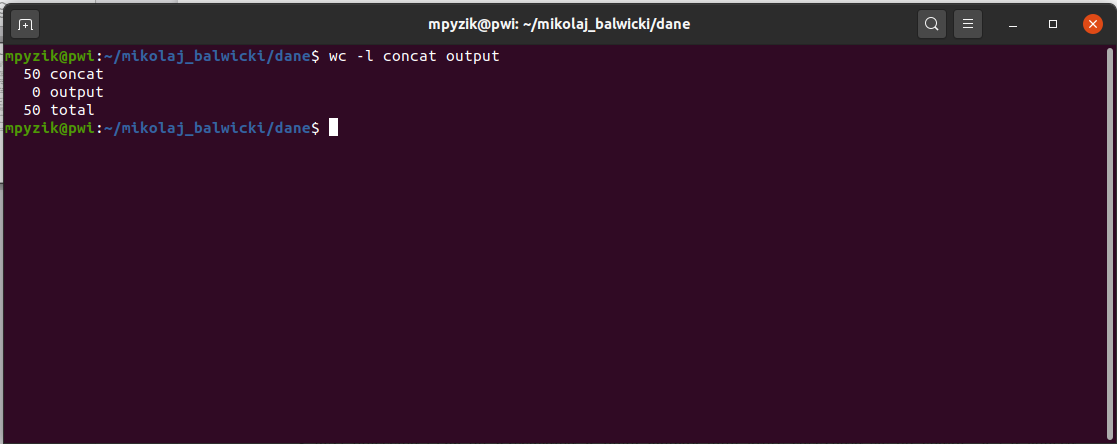
\includegraphics[width=\textwidth]{wc.png}

\end{document}
